\documentclass[a4paper, 12pt]{article}

\usepackage{graphicx}
\usepackage{float}
\usepackage{subcaption}

\graphicspath{{images/}}
\newcommand{\ie}{\textit{i}.\textit{e}., }
\newcommand{\eg}{\textit{e}.\textit{g}. }

\begin{document}

\title{LATEST RESEARCH DEVELOPMENTS IN RAM ARCHITECURE}
\date{}
\author{Masih Ahmed, 18117056, Btech 2nd year CSE}
\maketitle

\section{Introduction}
Conventional memory technologies are quickly approaching their physical limits and performance is saturating, inhibiting further development. In order to overcome this hurdle, the ultimate goal is to develop "universal memory" (UM), \ie a solution satisfying all the key requirements for a combined memory and storage device: cell size <4 $F^2$, read/write time <1 ns, write energy <1 fJ, endurance >$10^15$ , non-volatility with retention of more than ten years, and low cost for fabrication. 
\\
\\
\\
One such research breakthrough in RAM architecture is MeRAM which uses voltage-controlled magnetic anisotropy-magnetoelectric junctions (VCMA-MEJs) as memory elements and exploits a voltage-induced magnetization switching mechanism. The voltage-induced precessional switching can be ultra-fast (<1 ns), and has a switching energy down to ∼1 fJ, and the cell size of 4 $F^2$ with a diode access device; it is also non-volatile. The reason for the fast speed and low energy switching is that the interfacial perpendicular magnetic anisotropy (PMA) in CoFeB/MgO junctions can be modulated by applied voltage, causing precessional switching as shown in Fig,1 . This process ideally does not involve current flow for switching, therefore, the minimum energy per switch is limited only by the device capacitance $C$, and can ultimately reach ∼10 aJ given by ∼$CV^2$, where $V$ is the write voltage.

	\begin{figure}[H]
	\begin{center}
		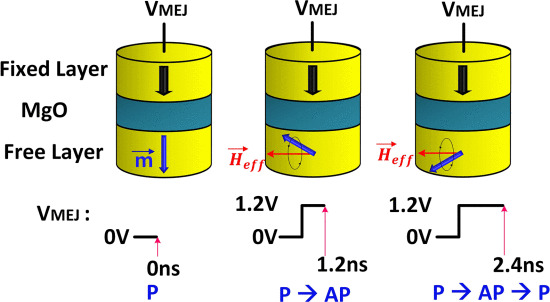
\includegraphics[scale=0.5]{Fig1.jpg}
		\caption {Precessional switiching process in MEJs}	
	\end{center}
	\end{figure}

\section{Background of VCMA-MEJ}
An MEJ consists of two ferromagnetic layers separated by a tunneling barrier MgO as shown in Fig. 1. The magnetic moment of one layer is able to change freely by using electrical and magnetic biases, and the other layer's magnetic moment is fixed. If the magnetic moments of the free and fixed layers are aligned in the same direction, the parallel state (denoted as P), the MEJ has a low resistance (R$_P$). In the anti-parallel state (denoted as AP), the free layer magnetization is in the opposite direction to the fixed layer, causing a high resistance ($R_AP$). Depending on the required speed of the reversal, switching of MEJs can be executed via precessional (also referred to as resonant) or thermally activated switching. Recent research has demonstrated VCMA switching in perpendicularly magnetized MEJs for both precessional and thermally activated regimes. The VCMA-MEJ effect can be explained by eletric-field-induces change of occupancy of atomic orbitals at inferace along with spin-orbit interaction. The VCMA-MEJ switching process is shown in Fig. 2 as follows. The PMA ($K_i$) is reduced by applying a voltage which with a correct polarity, lowers the energy barrier of the free layer. If the perpendicular anisotropy decreases sufficiently to remove the barrier due to the high enough applied voltage, switching can occur by a precessional reorientation of the magnetic moment. Even though the barrier is not sufficiently reduced, switching can also happen through thermal activation across the barrier.

	\begin{figure}[H]
	\begin{center}
		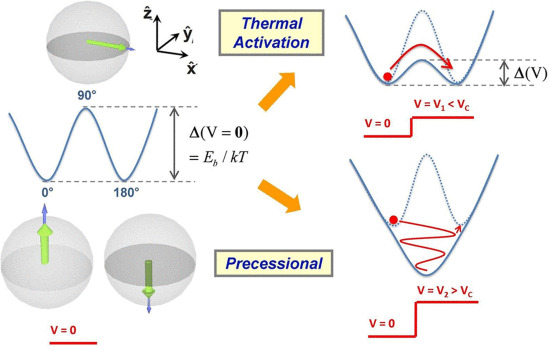
\includegraphics[scale=0.5]{Fig2.jpg}
		\caption {Description of VCMA-induced switching mechanism in PMA.}
	\end{center}	
	\end{figure}

\section{Emerging Memory Technologies With 1T-1R Cell Structure}
Comparing several types of emerging memory technologies and their performance with that of MeRAM in the form 1T-1R structure, \ie one access transistor associated with one resistive element, one can see that MeRAM outperforms in most of the categories as can be seen in Fig 3
\\
\\ PCRAM takes advantage of the resistance difference between the crystalline (low R) and amorphous (high R) states in phase change materials and has high retention, but the power and current hungry reset operation requires the access transistor to deliver high enough current, increasing its size.
\\
\\ReRAM has a relatively smaller write current compared to PCRAM and thus a smaller size, but it has low endurance $10^(5-8)$ and >10ns switching speed, limiting its applications
\\
\\In STT-RAM, switching operations are very fast, but due to high switching speed. an increase in write current is inevitable, requiring a larger transistor. Although it has unlimited endurance, the write energy is a formidable barrier to its practical usage.
\\
\\Due to the VCMA-driven precessional switching, MeRAM dramatically improves the write energy (down to ∼1 fJ/bit) and speed (<1 ns). Furthermore, it can be realized below a 10$F^2$ 1T-1MEJ structure, resulting from its very low write current of less than 10 $\mu$A. In addition, unlike STT-RAM, MeRAM is based on unipolar devices, which can exploit a conventional diode as an access device in a cell, hence, further reducing its cell size down to 4$F^2$, and enabling 3-D integration in the back-end of line process steps to achieve very high bit densities.
	
	\begin{figure}[H]
	\centering
		\begin{subfigure}[b]{0.5\linewidth}
			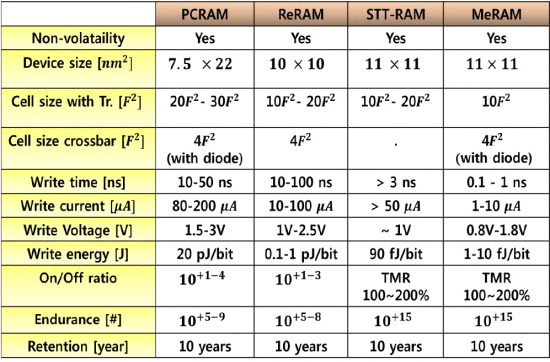
\includegraphics[scale=0.5]{Fig3.jpg}
		\end{subfigure}
		\begin{subfigure}[b]{0.5\linewidth}
			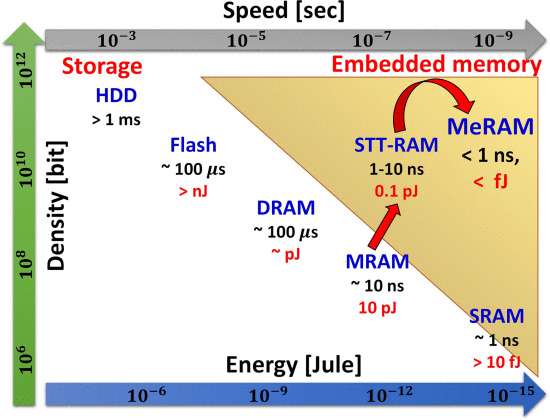
\includegraphics[scale=0.5]{Fig4.jpg}
		\end{subfigure}
		\caption {Comparision of emerging memory technologies.}
	\end{figure}

\end{document}

